\chapter{System Design}
\label{chap:design}

\section{Architectural Context}

CampusLoop supports the steps of a campus second-hand transaction, from publishing a listing and contacting another student to agreeing a price and confirming completion. The system divides this work between the browser, the backend, persistent storage, and services that provide advice. This division gives each component a clear responsibility while keeping the final transaction state under backend control.

The React browser client presents the pages and sends requests to FastAPI through JSON APIs. FastAPI checks whether the request is valid and whether the user may perform the action. PostgreSQL stores the resulting identities, listings, negotiations, orders, governance records, matching jobs, and audit evidence. Redis handles rate limiting and temporary state, while MinIO stores files and separates public product images from private chat and report evidence.

Some work runs outside an ordinary page request. A dedicated worker consumes matching jobs, and the M7/M8 advisory service provides versioned search, matching, price, trust, and risk rules through internal remote procedure calls (RPC). Figure~\ref{fig:architecture} shows how these components connect. The main distinction is that an advisory service can return a suggestion, but the API decides whether a business update is allowed and saves its result.

\begin{figure}[htbp]
  \centering
  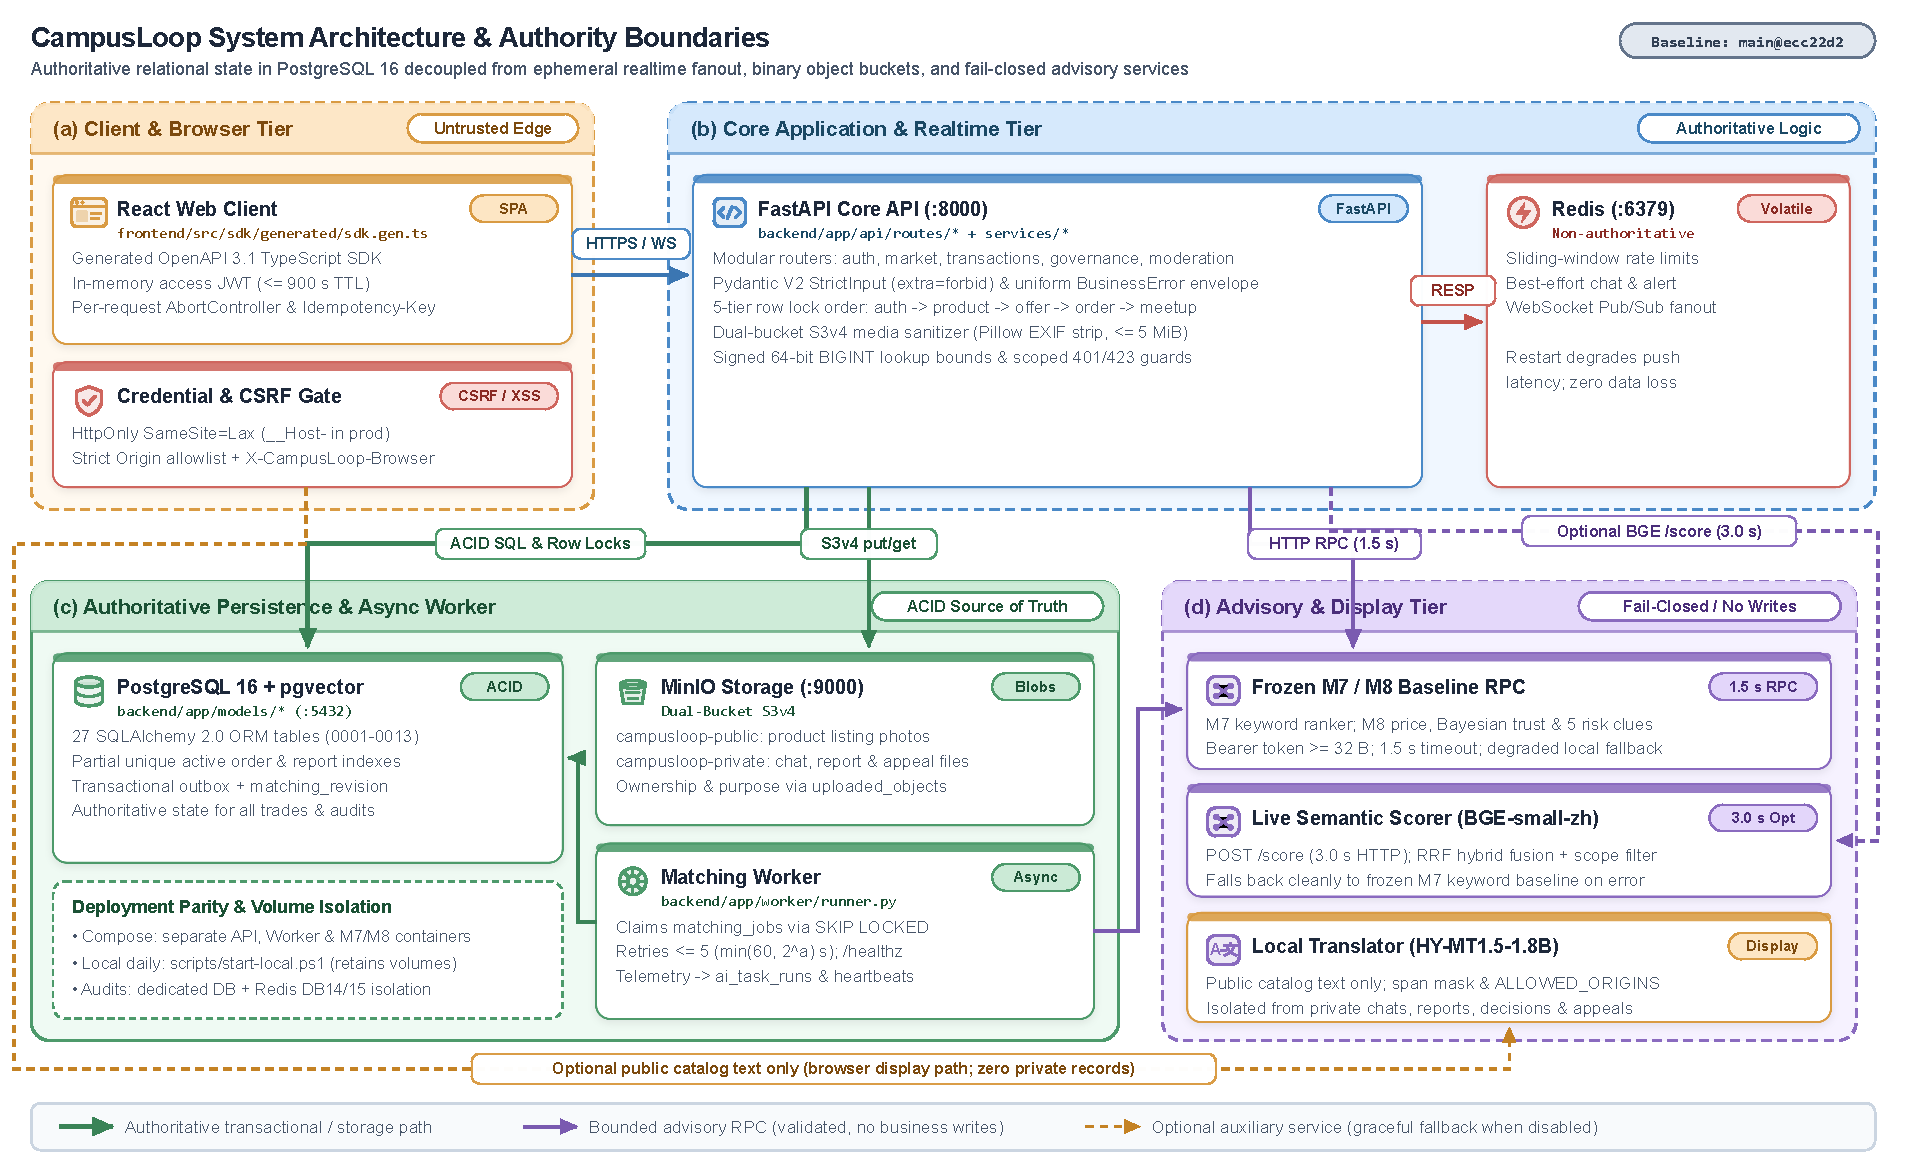
\includegraphics[width=\textwidth]{figures/design/architecture.pdf}
  \caption{CampusLoop runtime architecture and trust boundary.}
  \label{fig:architecture}
\end{figure}

This separation keeps advisory failures out of transaction updates. A timeout or malformed response from an advisory service must not mutate a product, accept an offer, complete an order, or resolve a report. The API performs business updates and commits them through PostgreSQL transactions. The repository's deployment configuration runs the API, worker, and advisory service as separate processes, with PostgreSQL, Redis, and MinIO as supporting services.

\section{Domain and Data Model}

The backend uses object-relational mapping (ORM) to describe database records as Python classes. Several classes share their timestamp columns through a Python mixin, consistent with SQLAlchemy's documented declarative-mixin mechanism~\cite{r2Mixins}. Class inheritance describes how the code reuses these attributes; foreign-key relationships describe how saved records refer to one another. The diagrams show these as separate relationships.

The data model follows the transaction journey. A \emph{User} owns products and wanted posts. A product or wanted post gives a two-party chat session its context, so a conversation remains linked to the item or request being discussed. Offers belong to that session. Accepting an offer creates an order for the referenced product, and the order retains its state history and at most one current meetup arrangement. A review can be submitted only after the transaction is completed.

Governance records serve a different purpose. A report refers to a user, product, order, or chat message and stores the reporter, evidence keys, resolution, handler, and timestamps. Separate AccountDecision and AccountAppeal records let students see account-handling decisions and request review without exposing private report contents.

The entity relationship diagram (ERD) is divided into catalog/chat, transaction, and governance views so that these relationships can be read without crowding one figure. Figure~\ref{fig:data-model} introduces the catalog and chat records. The figures show selected columns; the companion model/migration inventory gives all mapped columns, declared types, and migration constraints. Each record still has its own ownership and state rules.

\begin{figure}[htbp]
  \centering
  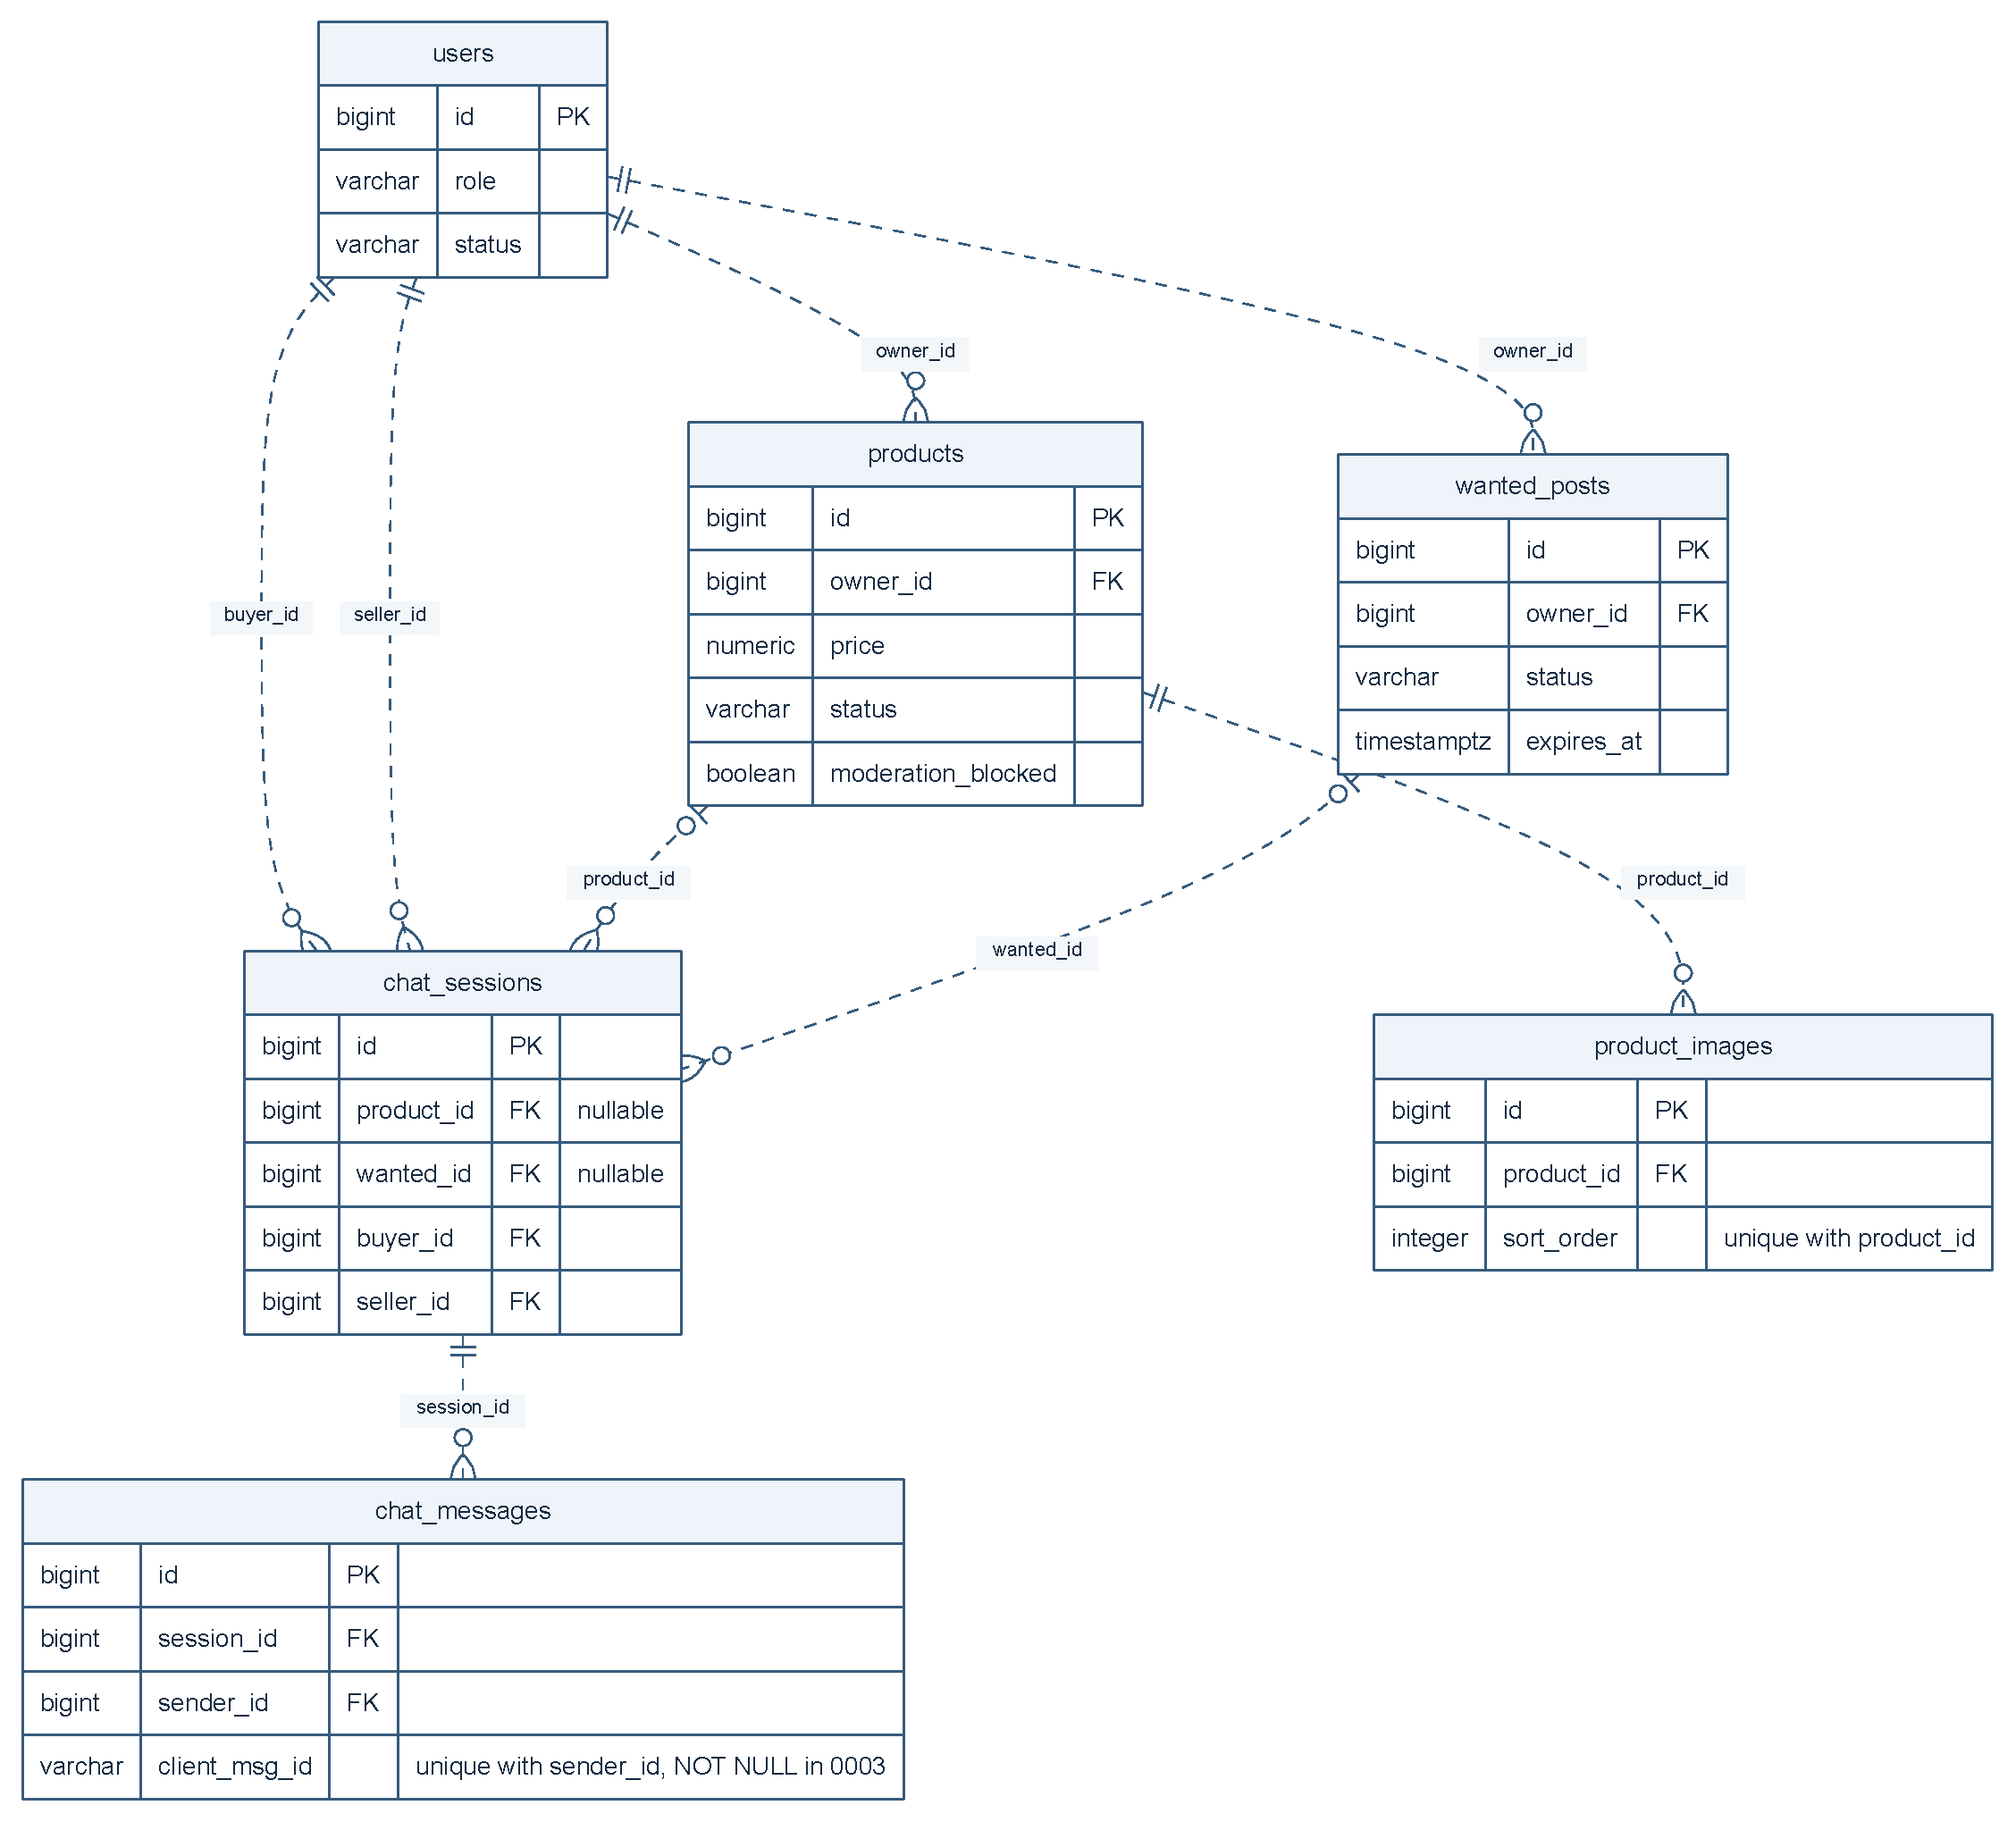
\includegraphics[width=\textwidth]{figures/design/data-model.pdf}
  \caption{Principal persistent entities and relationships.}
  \label{fig:data-model}
\end{figure}

Authentication records are separated from the user profile. A session family groups rotating refresh sessions and allows family-wide revocation after logout or replay detection. Matching jobs and matching results are also separate from live product records. The API therefore checks the live catalog for visibility and entity versions before returning ranked products.

\begin{figure}[p]
  \centering
  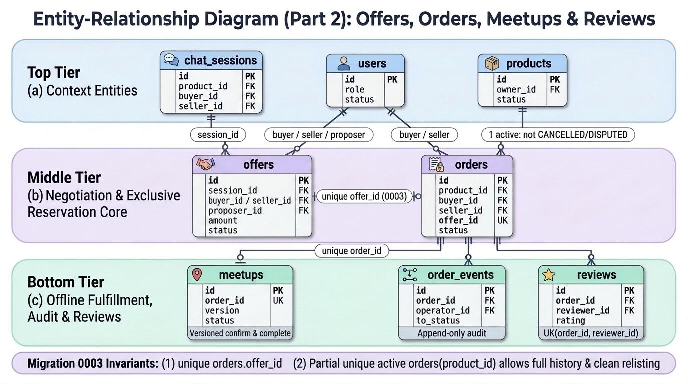
\includegraphics[width=\textwidth,height=0.8\textheight,keepaspectratio]{figures/design/data-model-transactions.pdf}
  \caption{Transaction ERD: historical orders and conditional reservation uniqueness.}
  \label{fig:erd-transactions}
\end{figure}
\begin{figure}[p]
  \centering
  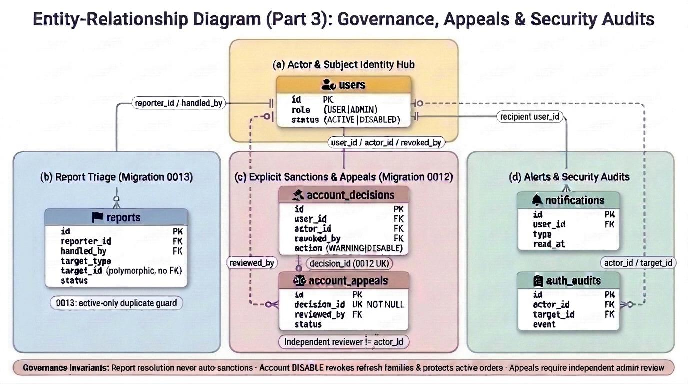
\includegraphics[width=\textwidth,height=0.8\textheight,keepaspectratio]{figures/design/data-model-governance.pdf}
  \caption{Governance ERD: reports, account decisions, appeals, and notifications.}
  \label{fig:erd-governance}
\end{figure}
\begin{figure}[p]
  \centering
  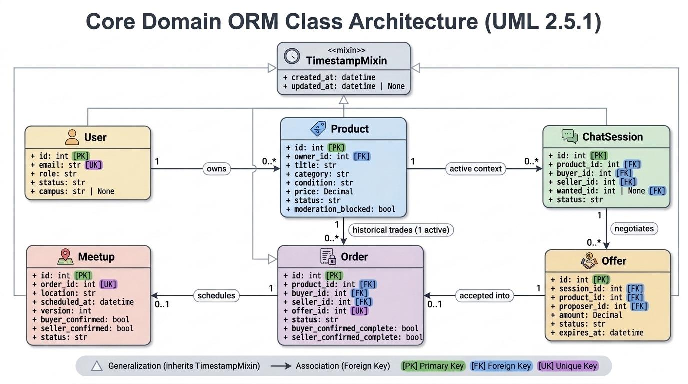
\includegraphics[width=\textwidth,height=0.8\textheight,keepaspectratio]{figures/design/class-diagram.pdf}
  \caption{Selected real ORM classes and their TimestampMixin inheritance.}
  \label{fig:class-diagram}
\end{figure}

Figures~\ref{fig:erd-transactions} and~\ref{fig:erd-governance} separate trading constraints from moderation records. Dashed Crow's Foot relationships are non-identifying foreign-key associations; circles mean optional participation and bars mean one. The class diagram in Figure~\ref{fig:class-diagram} shows selected mapped attributes and inheritance. Database constraints are recorded in the ERD and source inventory. Solid associations denote foreign-key references, not SQLAlchemy relationship objects. The selected classes declare no domain methods, so their diagram entries list attributes only. The source index records the exact definitions and the still-pending course-Lecture notation check.

\section{Authorization Boundaries}

The permission checks follow the relationship between a user and a record. A seller may edit an eligible product they own, while a conversation or order is accessible only to its participants. This means that being signed in does not give a user access to every record in the system.

These rules are enforced in backend routes and services. Student-only updates reject disabled or non-student actors. Product editing requires ownership and excludes reserved, sold, deleted, or moderated listings. Chat reads and writes require the actor to be either the buyer or seller, and wanted-match results are visible only to the wanted-post owner. Order operations require a participant; risk clues and report resolution require an administrator. Private files are read through authenticated API paths, while product media is placed in the public-read bucket.

The authentication path restores browser identity as follows. Login creates a server-side session family and returns an access token while the browser retains an opaque, HttpOnly cookie. On a page reload, the client calls \texttt{restoreBrowserSession}; the server validates the browser origin and cookie, applies the refresh window, records an audit event, and returns a new short-lived access token and current-user view. Refresh-token replay revokes the entire family before the API returns an authentication error.

\begin{figure}[htbp]
  \centering
  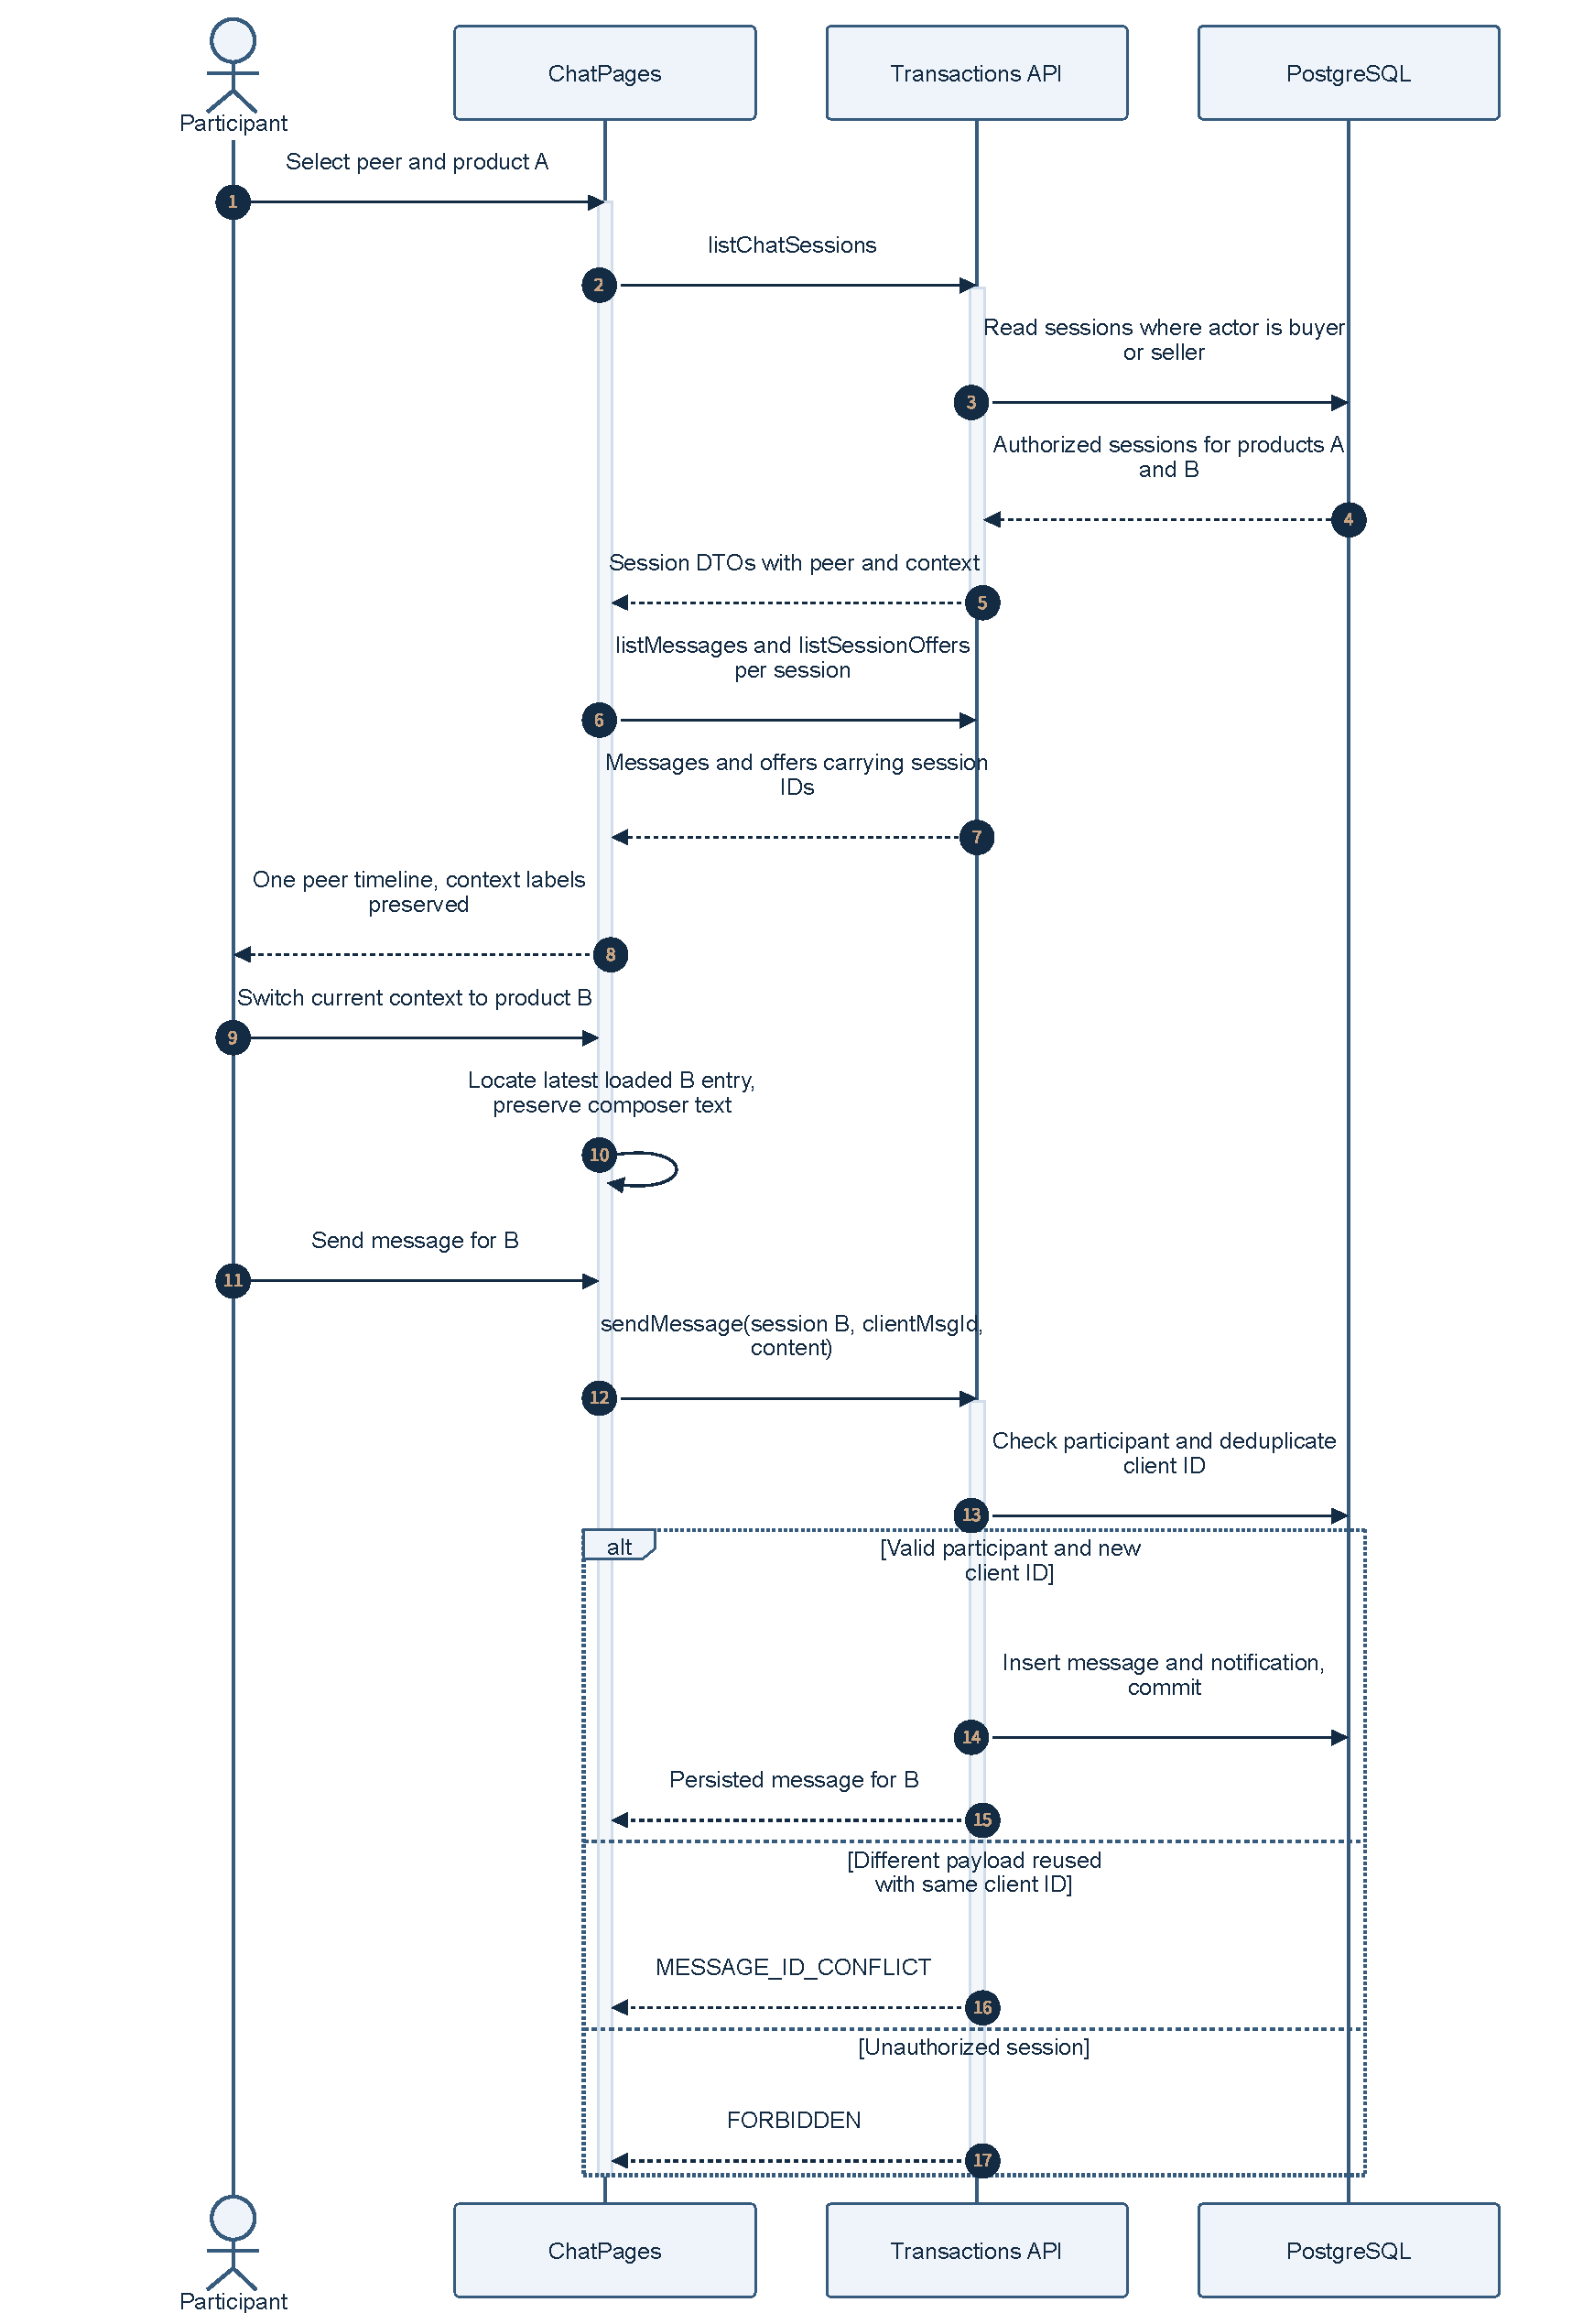
\includegraphics[width=0.94\textwidth]{figures/design/session-sequence.pdf}
  \caption{One peer timeline retaining separate product-session identities.}
  \label{fig:session-sequence}
\end{figure}

\section{Transaction State Machine}

A transaction changes both the order and the availability of the product. The API therefore updates their states together. When a pending offer is accepted under row locks, the product changes from \texttt{ON\_SALE} to \texttt{RESERVED}, and a new order enters \texttt{PENDING\_CONFIRM}. The reservation records that the item is involved in an agreed transaction, although the meeting and completion steps are still outstanding.

The participants then agree on a meetup proposal. Its version increases whenever the proposal changes, and a change resets both meetup confirmations and both completion confirmations. This matters because confirming an earlier time or place should not count as accepting a revised arrangement. The order reaches \texttt{MEETUP\_ARRANGED} only after both participants confirm the same version. It reaches \texttt{COMPLETED} only after both confirm completion against that version, at which point the product becomes \texttt{SOLD}. Figure~\ref{fig:transaction-states} shows this path.

\begin{figure}[htbp]
  \centering
  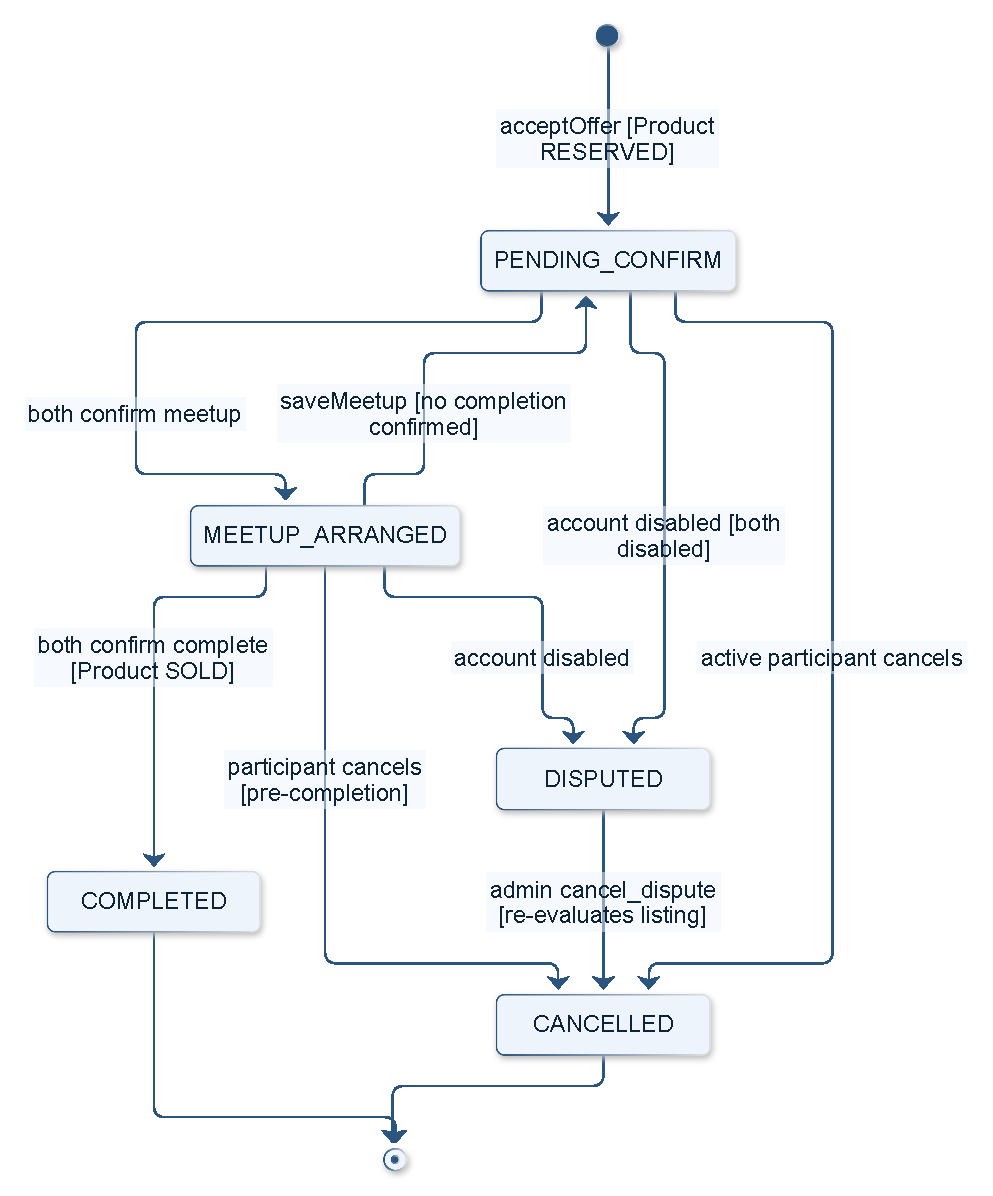
\includegraphics[width=0.94\textwidth]{figures/design/transaction-states.pdf}
  \caption{Coordinated listing, order, meetup, and completion states.}
  \label{fig:transaction-states}
\end{figure}

Cancellation depends on the order's state and confirmation flags. Once either participant has confirmed completion, cancellation is rejected. Before that point, cancellation releases an eligible listing back to \texttt{ON\_SALE}; a deleted or moderation-blocked listing remains \texttt{HIDDEN}. Every order transition appends an \texttt{OrderEvent}, preserving who acted, the before/after state, a description, and a timestamp. Figure~\ref{fig:order-meetup-sequence} shows the complete negotiation-to-completion interaction.

\begin{figure}[htbp]
  \centering
  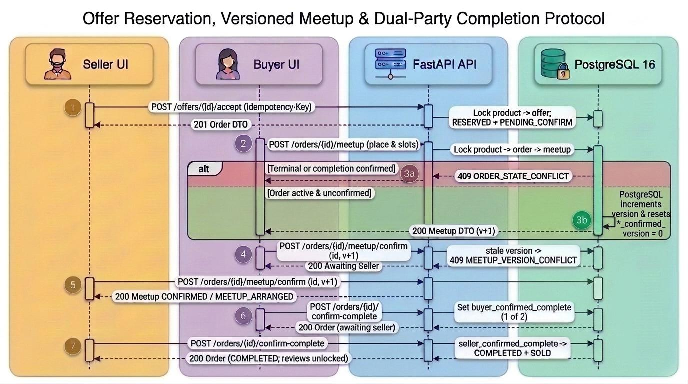
\includegraphics[width=\textwidth]{figures/design/order-meetup-sequence.pdf}
  \caption{Offer acceptance, versioned meetup agreement, and dual completion confirmation.}
  \label{fig:order-meetup-sequence}
\end{figure}

\section{Governance Design}

A report is a request for human review, not an automatic sanction. The reporting route prevents self-reporting, verifies that an order or chat-message reporter is a participant, verifies media ownership, and rejects a duplicate open report with the same reporter, target, and reason. Resolution is restricted to administrators. A normal decision accepts only pending or processing reports; changing a completed decision requires an explicit override containing the status and handling timestamp last observed by the administrator. The server compares those values with the saved record. A stale browser cannot overwrite a newer decision.

Each resolution saves the handler, time, required note, and resulting status. It also notifies the reporter and writes an audit event with before and after snapshots. The event explicitly records \texttt{enforcementExecuted=false}; the present implementation resolves the report record but does not claim that a user or listing sanction was automatically executed.

\section{Explicit Account Handling and Appeals}

Resolving a report records what an administrator decided about that report. Issuing a warning or disabling a student account is a separate action, which requires a reason, facts, and policy basis. Keeping these commands separate makes it possible to record the report outcome without silently treating it as an account sanction.

Disabling an account also affects transactions already in progress. The system revokes transaction sessions and protects the affected orders. Orders with a confirmed meetup or a completion confirmation move to dispute; earlier reservations remain available for controlled cancellation by an active participant. This treatment reflects the difference between an early reservation and a transaction where a participant may already have acted on an agreed meeting.

A student whose trading access is disabled can still use restricted appeal access to read the disclosed decision snapshot and submit an appeal. Another administrator normally reviews it. The development environment has an explicitly configured single-administrator exception, but its use is audited and does not count as independent review. If the account is reinstated, the original decision history remains, and disputed transactions are not automatically resolved.

\section{Traceability Baseline}

All claims in Chapters~\ref{chap:design}--\ref{chap:decisions} were checked against repository commit \texttt{edb9e32871eac2966750993294078acbfdba65f9}. The companion \texttt{architecture-source-index.md} maps every diagram and source chain to concrete routes, services, models, frontend calls, and deployment definitions. Using one fixed baseline keeps the chapter descriptions tied to the same version of the software.
